\documentclass[a4paper,12pt]{book}

\usepackage[latin1]{inputenc}
\usepackage[T1]{fontenc}
\usepackage[english]{babel}
\usepackage{url}
\usepackage{array}
\usepackage{lmodern}
\usepackage{fancyhdr}
\usepackage{graphicx}

\pagestyle{plain}

\title{\Huge{Klifehrian} \\ \large{Specifications}}
\author{K\'{e}vin \textit{''Linkyu''} \textbf{Guiraud} \\ Yannick \textit{''Zethzer''} \textbf{Bernard} \\ Masami \textit{''KexXie''} \textbf{Komuro} \\ Lo\"{i}s \textit{''Plopounet''} \textbf{Paulin}}
\date{\textbf{Last update :} \today}

\begin{document}
\maketitle
\thispagestyle{empty}
\setcounter{page}{0}
%-------------------------------------------------------------------------------------------
\part{General presentation}
%-------------------------------------------------------------------------------------------
%-------------------------------------------------------------------------------------------
\chapter{Presentation of Klifehrian}
%-------------------------------------------------------------------------------------------
\begin{itemize}
	\item Name : Klifehrian
	\item Type : Classic 2D RPG
	\item Style : Medieval fantasy
	\item Graphic style : ?
	\item Language, libraries, tools :
	\begin{itemize}
		\item C++
		\item OpenGL/SDL
		\item Tiled
	\end{itemize}
	\item Team :
%-------------------------------------------------------------------------------------------
	\begin{itemize}
		\item K\'{e}vin \textit{''Linkyu''} Guiraud
		\item Yannick \textit{''Zethzer''} Bernard
		\item Masami \textit{''KexXie''} Komuro
		\item Lo\"{i}s \textit{''Plopounet''} Paulin
	\end{itemize}
%-------------------------------------------------------------------------------------------
\end{itemize}
%-------------------------------------------------------------------------------------------
\newpage Insert here the life of Klifehrian and what's it.
%-------------------------------------------------------------------------------------------
\chapter{The Dream Team}
%-------------------------------------------------------------------------------------------
\section*{K\'{e}vin Guiraud}
Your presentation boss ;)

(yah yah I'll get around to that)

Blabla

Blabla

Blabla
%-------------------------------------------------------------------------------------------
\section*{Yannick Bernard}
\paragraph{Hi !} I'm twenty-two years old. I'm a undergraduate in Computer Sciences at the university Paul Sabatier in France. My passion for Computer Sciences time since the age of my 12 years. I started with a single computer and then from the age of 15, I began to study the IT in autodidact and I always continued since. I got my baccalaureat and started studies in IT at university.

In autodidact, I learned C, C++ later and finally the main web languages: HTML, CSS and PHP. I also learned the using of Debian distribution alone and amused myself on various mini- projects that have never really been finished.

For video games, it's different. On the anniversary of my 6 years old, my father offer me a Super Nintendo with Mario All Star, Mario Kart and Mario Paint. After That, my friends lent me several games including Sacred, Zelda 3, etc.

A few years later, I acquired a Playstation (the first!) in slim version. There I discovered the licence of Final Fantasy and I became a fan. With that, Gran Turismo, Tekken 3 (my first game on this console), etc

Then came the Playstation 2, the Devil May Cry marked me (I've bought in HD on Playstation 3for that matter).

At the same time, I had a computer with RTS like Age of Empires 2. I had internet access in 2007, which was rather late. But I did not waste my time to catch up on various mmorpg (Guild Wars 1 et 2, World of Warcraft, etc), RTS (Age of Empires 3 and Starcraft 2) and fps (Call of Duty, Battlefield , etc).

About Klifehrian, I'm the second member of the team \{.exe\}. For this game, I work essentially on the gameplay with K\'{e}vin, brainstorming and programmation. And I work on the annex activity, the card game : ''Insert a name''.

In a word, I am a geek.
%-------------------------------------------------------------------------------------------
\section*{Masami Komuro}
\paragraph{Hi there !} I was born on 1990.05.10 and I'm playing music as far as I could remember. I did C++, PHP and VB programming at school but my main occupation is music ! I'm part of the first team which started Klifehrian in 2007. Kevin relied on me to write and arrange music, and to create and design sound fx. At this time I worked with old synthesizers like Korg M1 and Yamaha TG77, so I programmed myself lot of patches in order to fit into the game mood.

I was so surprised when, in late 2013, Yannick and Kevin contacted me again to join the new Klifehrian Team : It meant Klifehrian would reborn ! So I accepted, and my work is now to provide high-quality audio and musics based on themes I wrote 6 years ago. The challenge is now to find all original scores and MIDI sequences (stored on floppies !!), but Original Klifehrian Music is not dead !
%-------------------------------------------------------------------------------------------
\section*{Lo\"{i}s Paulin}
Moi
%-------------------------------------------------------------------------------------------
%-------------------------------------------------------------------------------------------
%-------------------------------------------------------------------------------------------
\part{Game Engine}
%-------------------------------------------------------------------------------------------
%-------------------------------------------------------------------------------------------
\section*{What do we want?}
For the window size, we chose a resolution of 1024x692 pixels. If the display is set to be fullscreen, 2 black bands are displayed at the top and bottom; inside, some information of the game state, as, for example: characters' status, inventory, etc. (The player can change the displayed information).
\begin{itemize}
	\item The player can move in eight directions : up, down, left, right and diagonals. This implies a per-pixel configuration for moving.
	\item The player can interact with objects (chests, doors, ...), people, animals.
	\item The player can jump (in certain sections of the map only).
	\item The player can display the HUD when the game is in window mode with the HUD key (can be toggled between a "switch" or a "keep pressing" option). By default, the key used is [Alt].
	\item Collisions against :
	\begin{itemize}
		\item Walls (Houses, cliffs, ...)
		\item Trees
		\item Rocks
		\item People
		\item Objects
		\item Monsters
	\end{itemize}
\end{itemize}
The maps are created with Tiled and exported to XML for the 2D engine. See the gameplay part for specifics on the world of Klifehrian.
%-------------------------------------------------------------------------------------------
%-------------------------------------------------------------------------------------------
%-------------------------------------------------------------------------------------------
\part{Gameplay}
%-------------------------------------------------------------------------------------------
%-------------------------------------------------------------------------------------------
\chapter{Characters}
List of the playable characters in the game.
%-------------------------------------------------------------------------------------------
%-------------------------------------------------------------------------------------------
%-------------------------------------------------------------------------------------------
\section{Ren'D\^{u}r}
Main protagonist. Curly brown hair.
%-------------------------------------------------------------------------------------------
%-------------------------------------------------------------------------------------------
%-------------------------------------------------------------------------------------------
\section{Maeram}
Childhood friend. Ginger.
%-------------------------------------------------------------------------------------------
%-------------------------------------------------------------------------------------------
%-------------------------------------------------------------------------------------------
\section{Rufio}
Ren'D\^{u}r's best friend.
%-------------------------------------------------------------------------------------------
%-------------------------------------------------------------------------------------------
%-------------------------------------------------------------------------------------------
\section{Hezul}
Hybrid living in the forest north of Gutuid. Has joined a secret faction.
%-------------------------------------------------------------------------------------------
%-------------------------------------------------------------------------------------------
%-------------------------------------------------------------------------------------------
\section{Ran'Gor}
Historian mage.
%-------------------------------------------------------------------------------------------
%-------------------------------------------------------------------------------------------
%-------------------------------------------------------------------------------------------
\section{Gertan}
Wannabe knight, protector of the Darez.
%-------------------------------------------------------------------------------------------
%-------------------------------------------------------------------------------------------
%-------------------------------------------------------------------------------------------
\section{Yasoi}
Warrior wielding the greataxe, she's set to kill the most demons she can.
%-------------------------------------------------------------------------------------------
%-------------------------------------------------------------------------------------------
%-------------------------------------------------------------------------------------------
%-------------------------------------------------------------------------------------------
\chapter{World}
\begin{figure}[h]
	\centering
		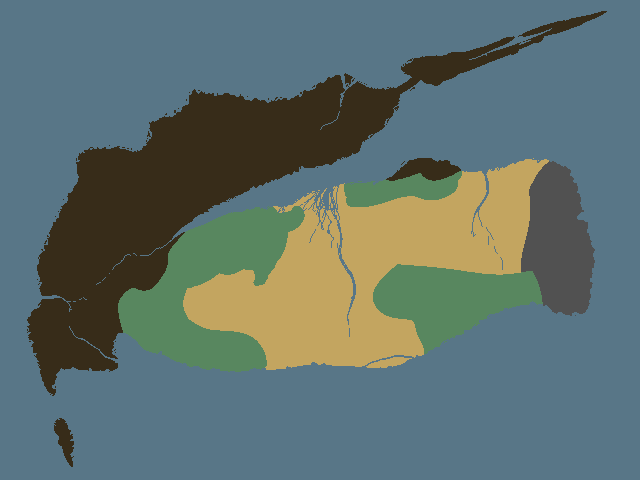
\includegraphics[scale=2]{worldmap.png}
	\caption{Map of Klifehrian}
	\label{fig:worldmap}
\end{figure}
%-------------------------------------------------------------------------------------------
%-------------------------------------------------------------------------------------------
%-------------------------------------------------------------------------------------------
\section{Towns}
\begin{figure}[h]
	\centering
		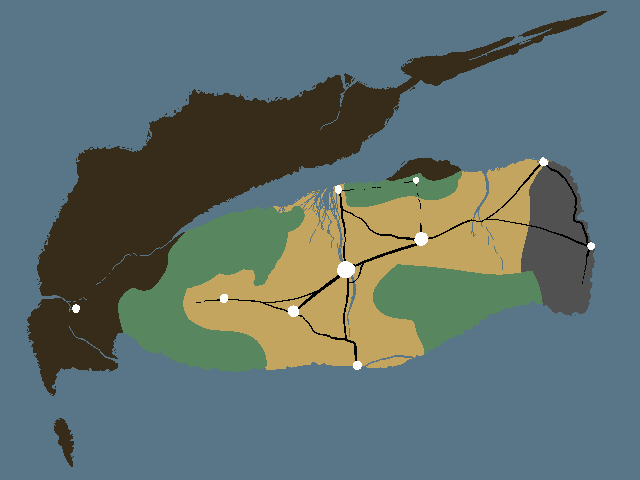
\includegraphics[scale=2]{worldmap_cities.png}
	\caption{Map of Klifehrian with the cities and roads}
	\label{fig:worldmap_cities}
\end{figure}
%-------------------------------------------------------------------------------------------
%-------------------------------------------------------------------------------------------
\subsection{Terdal}
Ren'D\^{u}r and Maeram's hometown; this is where the adventure starts.
%-------------------------------------------------------------------------------------------
%-------------------------------------------------------------------------------------------
\subsection{Danlemaup}
Festive city and crossroads of the continent.
%-------------------------------------------------------------------------------------------
%-------------------------------------------------------------------------------------------
\subsection{Unnamed town}
A town I put between Danlemaup and Terdal but forgot all about it. Probably gonna make it be a small town of some sort.
%-------------------------------------------------------------------------------------------
%-------------------------------------------------------------------------------------------
\subsection{Kalum Harbor}
A big fishing harbor that eventually became a city.
%-------------------------------------------------------------------------------------------
%-------------------------------------------------------------------------------------------
\subsection{Felsy Creek}
Small harbor located north of Danlemaup.
%-------------------------------------------------------------------------------------------
%-------------------------------------------------------------------------------------------
\subsection{Gutuid}
Capital. Fortified.
%-------------------------------------------------------------------------------------------
%-------------------------------------------------------------------------------------------
\subsection{Waldenia}
Large camp in the forest. Base of the Silver Blades.
%-------------------------------------------------------------------------------------------
%-------------------------------------------------------------------------------------------
\subsection{Remisci}
A small city on the far east. Currently in a deadlock with the demons.
%-------------------------------------------------------------------------------------------
%-------------------------------------------------------------------------------------------
\subsection{Bergwork}
A mine that is now the stronghold of all demons.
%-------------------------------------------------------------------------------------------
%-------------------------------------------------------------------------------------------
%-------------------------------------------------------------------------------------------
\section{PNJs}
Bla
%-------------------------------------------------------------------------------------------
%-------------------------------------------------------------------------------------------
%-------------------------------------------------------------------------------------------
\section{Combat}
The combat are mainly in a Golden Sun style, except the ATB jauge in a Grandia style.
%-------------------------------------------------------------------------------------------
%-------------------------------------------------------------------------------------------
%-------------------------------------------------------------------------------------------
\section{Bestiary}
Bla
%-------------------------------------------------------------------------------------------
%-------------------------------------------------------------------------------------------
\subsection{MonsterType 1}
Bla
%-------------------------------------------------------------------------------------------
\subsubsection{Monster 1}
Bla
%-------------------------------------------------------------------------------------------
\subsubsection{Monster 2}
Bla
%-------------------------------------------------------------------------------------------
%-------------------------------------------------------------------------------------------
\subsection{MonsterType 2}
Bla
%-------------------------------------------------------------------------------------------
\subsubsection{Monster 1}
Bla
%-------------------------------------------------------------------------------------------
\subsubsection{Monster 2}
Bla
%-------------------------------------------------------------------------------------------
%-------------------------------------------------------------------------------------------
\subsection{MonsterType 3}
Bla
%-------------------------------------------------------------------------------------------
\subsubsection{Monster 1}
Bla
%-------------------------------------------------------------------------------------------
\subsubsection{Monster 2}
Bla
%-------------------------------------------------------------------------------------------
%-------------------------------------------------------------------------------------------
%-------------------------------------------------------------------------------------------
%-------------------------------------------------------------------------------------------
\chapter{UI}
%-------------------------------------------------------------------------------------------
%-------------------------------------------------------------------------------------------
%-------------------------------------------------------------------------------------------
\section{Menu}
It's important in the game. You can see the current team, time, money and a list of actions. \\ Illustration of menu when you get it done: \\ ''Insert image here''
%-------------------------------------------------------------------------------------------
%-------------------------------------------------------------------------------------------
\subsection{Inventory}
No limit for the weight. Each character has his own inventory. All characters can equip every types of equipment. It is possible to have an exchange of objects between characters. It is possible to sort objects by name and type. For that, we must be in the inventory of one character. \\
See section 5.4 for bank.
See section 5.5 for caravan.
\textbf{Description of the inventory :} On the left we can choose the character. When the cursor is on the avatar, we see the inventory. To select an object, we select the character. After selecting the character and the object, a little window appear with:
\begin{itemize}
	\item Use
	\item Exchange
\end{itemize}
See section 4.3 for inventory in combat.
Illustration : \\ ''Insert image here''
%-------------------------------------------------------------------------------------------
%-------------------------------------------------------------------------------------------
\subsection{Stats}
\textbf{Levels of the character :} 1 to 100 \\
\textbf{Levels of one skill :} 1 to 3 \newpage (For instance : Fire lv.1 => Fire lv.2 => Fire lv.3)
\begin{itemize}
	\item Strength : for physical power
	\item Intellect : for magic power
	\item Stamina : for life
	\item Agility : for dodging, critical rate, and ATB speed
	\item Defense : influenced by the equipment only
\end{itemize}
%-------------------------------------------------------------------------------------------
%-------------------------------------------------------------------------------------------
\subsection{Team}
Bla
%-------------------------------------------------------------------------------------------
\subsection{Equipment}
Bla
%-------------------------------------------------------------------------------------------
%-------------------------------------------------------------------------------------------
\subsection{Skills}
Complete list of skills. At the top is a window with the characters' avatars. The avatar of the selected character appears colored while the others are grayed out. \\ Illustration : \\ ''Insert image here''
%-------------------------------------------------------------------------------------------
%-------------------------------------------------------------------------------------------
\subsection{Specialization}
There are three specializations: melee, magic and dexterity. Each character can choose one and only one. This will change the ratio of its statistics. It can change as many times as he wants when out of combat. In combat: see section 4.3.
In the menu, the cursor comes on the character window. You select the character and a little window appears with the three specializations. \\ Illustration : \\ ''Insert image here''
%-------------------------------------------------------------------------------------------
\subsubsection{Melee}
Specialization ''melee'' allows a character to be based on physical skills and strong endurance. It's ideal for taking many hits and it has a slow but powerful attack. \newpage
Ratio :
\begin{itemize}
	\item Strength : 2
	\item Stamina : 1
	\item Agility : 0.75
	\item Intellect : 0.5
\end{itemize}
%-------------------------------------------------------------------------------------------
\subsubsection{Magic}
Specialization ''magic'' allows a character based on magical abilities and with low endurance. It will be privileged to support the team and has a panel of magical skills moderately slow but powerful. \\
Ratio :
\begin{itemize}
	\item Strength : 0.75
	\item Stamina : 0.5
	\item Agility : 1
	\item Intellect : 2
\end{itemize}
%-------------------------------------------------------------------------------------------
\subsubsection{Dexterity}
Specialization ''dexterity'' allows a character based on physical skills and an average endurance. It will be ideal for dealing fast damage to the enemy and has a panel of quick and powerful medium to very powerful physical skills. It is the only one able to use the skills of thievery. \\
Ratio :
\begin{itemize}
	\item Strength : 1
	\item Stamina : 0.75
	\item Agility : 2
	\item Intellect : 0.5
\end{itemize}
%-------------------------------------------------------------------------------------------
%-------------------------------------------------------------------------------------------
\subsection{Skills list}
The cursor comes on the character. The player pick one and the window changes. Top left, it has the character's avatar. Using the full height of the screen on the right: the list of skills already activated for this character \textbf{(NUMBER TO DEFINE)}. On the left (under the avatar and slightly more on the left of it), the total list of skills. \\ Illustration : \\ ''Insert image here''
%-------------------------------------------------------------------------------------------
%-------------------------------------------------------------------------------------------
\subsection{Options}
The options of the game.
%-------------------------------------------------------------------------------------------
%-------------------------------------------------------------------------------------------
%-------------------------------------------------------------------------------------------
\section{Skill system}
\textbf{To learn a skill:} The character must wear the equipment that has the competence on it. The more the character fights, the more SP (Skill Points) he gains on the skill. While learning, if the equipment is worn, the character can use the skill. To use it without the equipment, it must be fully learned. If the monster is more powerful than the character, level-wise, he earns more SP. Some skills can not be learned if the player does not have the required level. The equipment may be equipped, but with a penalty. \\
\textbf{To increase the level of skills:} To level up a skill, the character must use the skill. The more he uses it, the more it will increase the level of the skill. The skill will gain experience from its use. \textbf{(FORMULA TO DEFINE)} \\
\textbf{Special skills:} Skills that are specific to a character; each character has one special skill for each specialization.
%-------------------------------------------------------------------------------------------
%-------------------------------------------------------------------------------------------
\subsection{Magic}
Bla
%-------------------------------------------------------------------------------------------
\subsubsection{Skill 1}
Bla
%-------------------------------------------------------------------------------------------
\subsubsection{Skill 2}
Bla
%-------------------------------------------------------------------------------------------
%-------------------------------------------------------------------------------------------
\subsection{Physical}
Bla
%-------------------------------------------------------------------------------------------
\subsubsection{Skill 1}
Bla
%-------------------------------------------------------------------------------------------
\subsubsection{Skill 2}
Bla
%-------------------------------------------------------------------------------------------
%-------------------------------------------------------------------------------------------
\subsection{Invocations}
Bla
%-------------------------------------------------------------------------------------------
\subsubsection{Invocation 1}
Bla
%-------------------------------------------------------------------------------------------
\subsubsection{Invocation 2}
Bla
%-------------------------------------------------------------------------------------------
%-------------------------------------------------------------------------------------------
\subsection{Passive}
Bla
%-------------------------------------------------------------------------------------------
\subsubsection{Passive 1}
Bla
%-------------------------------------------------------------------------------------------
\subsubsection{Passive 2}
Bla
%-------------------------------------------------------------------------------------------
%-------------------------------------------------------------------------------------------
%-------------------------------------------------------------------------------------------
\section{Objects}
In the game, can be found different items. The player can get objects from chests, monsters after a combat, etc. The objects can be stored in the inventory, the bank and the caravan.
For role play purposes, the objects dropped by monsters respect that rule : Monsterkind drop. For example, you can't find money on a wolf, but a wolf hide, wolf meat and wolf teeth (human skin is hard for young people, so you can't find it too).
Report to section 5.1.1 for the inventory.
Report to section 5.4 for the bank.
Report to section 5.5 for the caravan.
With the equipment, report to section 5.2 for learning skill.
%-------------------------------------------------------------------------------------------
%-------------------------------------------------------------------------------------------
\subsection{ObjectType 1}
Bla
%-------------------------------------------------------------------------------------------
\subsubsection{Object 1}
Bla
%-------------------------------------------------------------------------------------------
\subsubsection{Object 2}
Bla
%-------------------------------------------------------------------------------------------
\subsubsection{Object 3}
Bla
%-------------------------------------------------------------------------------------------
%-------------------------------------------------------------------------------------------
\subsection{ObjectType 2}
Bla
%-------------------------------------------------------------------------------------------
\subsubsection{Object 1}
Bla
%-------------------------------------------------------------------------------------------
\subsubsection{Object 2}
Bla
%-------------------------------------------------------------------------------------------
\subsubsection{Object 3}
Bla
%-------------------------------------------------------------------------------------------
%-------------------------------------------------------------------------------------------
\subsection{ObjectType 3}
Bla
%-------------------------------------------------------------------------------------------
\subsubsection{Object 1}
Bla
%-------------------------------------------------------------------------------------------
\subsubsection{Object 2}
Bla
%-------------------------------------------------------------------------------------------
\subsubsection{Object 3}
Bla
%-------------------------------------------------------------------------------------------
%-------------------------------------------------------------------------------------------
%-------------------------------------------------------------------------------------------
\section{Bank system}
Bla
%-------------------------------------------------------------------------------------------
%-------------------------------------------------------------------------------------------
%-------------------------------------------------------------------------------------------
\section{Caravan system}
Bla
%-------------------------------------------------------------------------------------------
%-------------------------------------------------------------------------------------------
%-------------------------------------------------------------------------------------------
%-------------------------------------------------------------------------------------------
\chapter{The card game: ''Insert a name''}
This card game is an minor activity in the game. The player can play that or not. However, the ''Legendary Card'' does interfere with the game.
%-------------------------------------------------------------------------------------------
\section{Specifications:}
\begin{itemize}
	\item 40 cards maximum in the deck
	\item \textbf{Number to define} cards in the game
	\item 1 vs 1
	\item 25 health points per player
	\item Maximum of 3 identical monster cards in the deck.
	\item Maximum of 2 identical trap cards in the deck.
	\item Maximum of 2 identical instant cards in the deck.
\end{itemize}
%-
\textbf{Cards type:}
\begin{itemize}
	\item Monsters : \textbf{Types to define}
	\item Traps : Never attack the player directly
	\item Instants : Never attack the health points of the player directly
\end{itemize}
%-
\textbf{Rarity level:}
\begin{itemize}
	\item Common: The player can buy them to a specific NPC. He can win those cards against NPC Players. And he can find them in chests.
	\item Rare: The player can win them against NPC players. They can also be found in chests.
	\item Legendary: Can only be stolen on specific bosses (which means the player need a dexterity-oriented character in his team). He can also find: 1 instant card in a chest and 1 trap card in a other chest (quest chain for both of those).
\end{itemize}

%-------------------------------------------------------------------------------------------
\section{Rules:}
\subsection{Game procedures}
\begin{enumerate}
	\item Each player pick 7 cards (7 cards maximum in the hand. Otherwise, the player discards cards until they have 7 left)
	\begin{itemize}
		\item The player picks a card when it's their turn.
	\end{itemize}
		\item One color per player : Red and Blue. A coin is tossed to see who starts.
		\item The chosen player starts (whose turn it is):
	\begin{itemize}
		\item Case A : The player puts down a monster card. (The monster card cannot attack when it's put down)
		\item Case B : The player puts down a trap card face down.
		\item NB : The player can do ''Case A'' or ''Case B''
		\item Case C : The player puts down a monster card and a trap card face down.
		\item NB : The ''Case C'' is forbidden in the first two turns. (Explanation : The first player play, after the second and now, it's third turn time)
		\item Case D : The player want to play an instant card. It's forbidden in the first two turns.
		\item NB : So, each player in the first two turns have : One monster card or one trap card (face down).
	\end{itemize}
	\item When it's the third turn (Explanation : Each player play one card), we can have a attack/defense phase.
\item After the third turn, the case A, B, C or D can apply. And we continue until a player loses all their health points.
\item \textbf{IMPORTANT : The player disengages their card when it's their turn.}
\end{enumerate}
%---
\subsubsection{Attack/Defense phase}
\begin{itemize}
	\item A single instant card can be played.
	\item An attacking monster engages (the card rotates 90 degrees)
	\item A engaged monster cannot defend.
		\begin{itemize}
			\item A monster can be engaged for only its effect. (If it's for that, it can't attack)
			\item A monster attacks only one card.
			\item Several monsters can attack the same card.
		\end{itemize}
	\item Defending monsters don't engage.
	\item If there are several monsters against one:
		\begin{itemize}
			\item If the first attacking monster kills the monster. The second attacks into the void. The player wastes the attack and the monster stays engaged.
			\item Else the first and second (and more) attacks the defending monster.
				\begin{itemize}
					\item If the defending monster is still alive. Possibility :
					\begin{itemize}
						\item Case A : Add an other monster for attacking (the monster is engaged for that).
						\item Case B : Use an instant card.
					\end{itemize}
					\item Else, the defending monster is dead.
				\end{itemize}
		\end{itemize}
\item Else, we have a 1 vs 1:
	\begin{itemize}
	\item If the defending monster is still alive. Possibility :
	\begin{itemize}
		\item Case A : Add an other monster for attacking (the monster is engaged for that).
		\item Case B : Use an instant card.
	\end{itemize}
	\item Else, the defending monster is dead.
	\end{itemize}
\item NB : A trap card is triggered when the attacking monster attacks if the trap card does an effective effect for that.
\item NB : A trap card can counter an instant card if the effect of the card permit that.
\item NB : An instant card is played :
	\begin{itemize}
		\item Before the attack
		\item After the attack
		\item For defending if the defending plyer doesn't have a trap card or with a trap card.
		\item \textbf{IMPORTANT : One instant card per turn}
	\end{itemize}
\end{itemize}
%---
\subsubsection{End of the party}
\begin{itemize}
\item The party is over when one player have his health points down to 0 (or less).
\item If the player (the IRL player) wins the party. They wins a card from the NPC.
	\begin{itemize}
		\item Possibility to play against almost all of the NPCs of Kliferhian.
			\begin{itemize}
				\item Several NPCs have the common cards.
				\item In Kliferhian, the player will have to search for specific NPCs for certain rare cards.
			\end{itemize}
	\end{itemize}
\end{itemize}
%---
%---
\section{Damage range}
\subsection{Extremums :}
\begin{itemize}
\item 0/5 (Defensive only with an effect for attacking. Legendary Card)
\item 5/0 (Attack only with an effect for defense. Legendary Card)
\item 5/5 (Legendary. Unique card. The player finds that card on an optional boss near the end of the game.)
\end{itemize}
\newpage
\subsection{Other damage :}
\begin{itemize}
	\item Commons :
	\begin{itemize}
		\item 1/0
		\item 1/1
		\item 2/1
		\item 1/2
		\item 2/2
		\item 0/2 (Defense without effect)
		\item 0/3 (Defense without effect)
	\end{itemize}
	\item Rare :
	\begin{itemize}
		\item 3/1
		\item 1/3
		\item 2/3
		\item 3/2
		\item 3/3
		\item 0/2 (Defense with effect)
		\item 0/3 (Defense with effect)
	\end{itemize}
	\item Legendary :
	\begin{itemize}
		\item 4/2
		\item 4/3
		\item 3/4
		\item 5/3
		\item 5/2
		\item 2/5 
		\item 3/5
		\item 4/4
		\item 0/4 (Defense with effect)
	\end{itemize}
\end{itemize}
%---
%---
\newpage
\section{List of cards}
This list is not definitive.
\subsection{Monsters}
\textbf{Bestiary to do first !}
%--
\subsection{Trap cards}
\begin{itemize}
	\item Commons :
	\begin{itemize}
		\item Paralyzes the monster for 1 turn
		\item Paralyzes the monster for 2 turn
		\item Suppression of the monster until end of turn
		\item Returns the monster in the hand of his opponent
		\item Removes 1 health point from the monster
		\item Removes 2 health points from the monster
		\item Engages an other monster on the battlefield (the defending player chooses)
		\item ...
	\end{itemize}
	\item Rare :
	\begin{itemize}
		\item Paralyzes the monster for 3 turn
		\item Kills the monster card (Unique card)
		\item Removes 3 health points from the monster
		\item Engages all monsters of of the opponent (Unique card)
		\item ...
	\end{itemize}
	\item Unique legendary card :
	\begin{itemize}
		\item Kills all monsters of the opponent
	\end{itemize}
\end{itemize}
%--
\subsection{Instant cards}
\begin{itemize}
	\item Commons :
	\begin{itemize}
		\item The opponent discards 1 card (Chosen by the caster)
		\item The opponent discards 2 cards (Chosen by the caster)
		\item Cancels the attack of an attacking monster
		\item Removes 1 health point from a targetted monster (attack or not)
		\item Removes 2 health points from a targetted monster (attack or not)
		\item Engages an opponent's monster
		\item ...
	\end{itemize}
	\item Rare :
	\begin{itemize}
		\item The opponent discards 3 cards (Chosen by the caster)
		\item Cancels the attack of 2 attacking monsters
		\item Cancels the attack of all attacking monsters (Unique card)
		\item Removes 3 health points from a targetted monster (attack or not)
		\item Resurrects a monster from your own cemetery
		\item Resurrects a monster from the opponent's cemetery and takes the control of it (Unique card)
		\item Picks up an instant card or a trap card from your own cemetery
		\item ...
	\end{itemize}
	\item Unique legendary card :
	\begin{itemize}
		\item Removes all cards from opponent's battlefield
	\end{itemize}
\end{itemize}
%---
%---
\newpage
\section{Schema of the game board}
\begin{figure}[h]
	\centering
		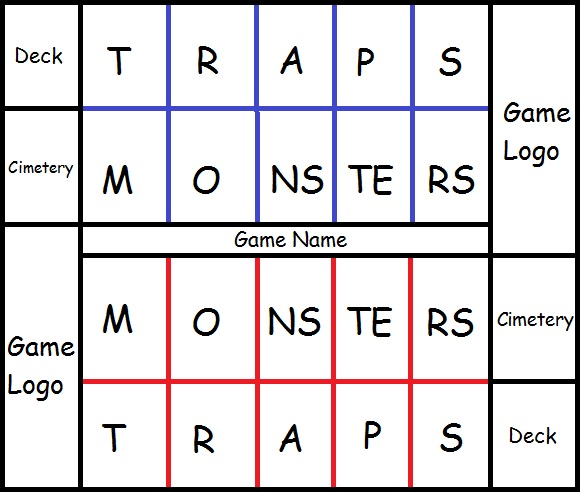
\includegraphics{gameboardcard.jpg}
	\caption{Schema of the game board}
	\label{fig:gameboardcard}
\end{figure}

%-------------------------------------------------------------------------------------------
%-------------------------------------------------------------------------------------------
%-------------------------------------------------------------------------------------------
\part{Music}
\chapter{What do we feel the player?}
Klifehrian original themes composition was started circa february 2007. At this time, the project was developed on RPG MAKER platform, which only supports Audio or General MIDI loop tracks. So, original Klifehrian soundtrack was originally projected as GM sequences, and a few moment later, as audio tracks (made from MIDI sequences rendered on custom-programmed professional synthesizers).
\\ \\
Now, 7 years later, the big challenges are the following :
\begin{itemize}
	\item Organize musical themes by reanalyzing original MIDI sequences.
	\item Write some additional themes
	\item Think about the ways for dynamically embedding audio segments into the game.
	\item Arrange, record, mix those elements.
\end{itemize}
Main musical axes written in 2007 are the following :
\begin{itemize}
	\item Klifehrian melody
	\item Kren'd\^ur Theme
	\item Rufio Theme
	\item Ending Bonus Song
\end{itemize}
\newpage Beside this, there were several musics which were associated with events \/ functions :
\begin{itemize}
	\item 4 battle themes (2 really used)
	\item 3 spooky \/ horror themes
	\item victory \/ fail musics
	\item Character Theme spin-offs used as event music.
\end{itemize}
The new organization for music writing into Klifehrian is easy to plan, using a simple grid.
Horizontally, the theme (melody) is chosen according to the character, or the action actor (subject) ; whereas, vertically, the background (orchestration, variation) is based on the environment and the circumstances of the scene (object).
\\ \\
\begin{tabular}{|>{\centering \arraybackslash}p{3cm}|>{\centering \arraybackslash}p{3cm}|>{\centering \arraybackslash}p{3cm}|>{\centering \arraybackslash}p{3cm}|}
\hline
 & \textbf{Kren'd\^ur} & \textbf{Rufio} & \textbf{Maeram} \\ 
\hline
\textbf{Town A} & seq T1A & - & - \\
\hline
\textbf{Town B} & seq T1B & - & - \\
\hline
\textbf{Map A} & - & - & - \\
\hline
\textbf{Map B} & - & - & - \\
\hline
 \textbf{...} & seq ... & seq ... & seq ... \\
\hline
\end{tabular}
\\ \\ \\
A notable exception is for battle musics. Two strategies are available :
\begin{enumerate}
	\item Theme depends of player-controlled character, arrangement is based on the enemy (AI-controlled)
	\item Theme and melody are associated with the enemy, arrangement depends of player-controlled character. 
\end{enumerate}
Arrangement can optionally evolve according to one of the battler's life gauge. It's also possible to use conditional loopings. This subject will be developed later into the appropriate section (7.1.3)
%------------------------------------------------------------------------------------------------------------------------------------
%------------------------------------------------------------------------------------------------------------------------------------
\section{World}
Blo
\subsection{Towns}
Blo
\subsection{Maps}
Blo
\subsection{Combat}
Blo
%------------------------------------------------------------------------------------------------------------------------------------
%------------------------------------------------------------------------------------------------------------------------------------
\section{UI}
Blo
\subsection{Titlescreen}
Blo
\subsection{Credits}
Blo
\end{document}